\documentclass[12pt]{article}
\usepackage{fancyhdr}
\pagestyle{fancy}
\fancyhf{}
\fancyfoot[C]{\thepage}
\fancyfoot[L]{\scriptsize CC BY-NC-SA 4.0 \textbullet\ Leo Liang}
\renewcommand{\headrulewidth}{0pt}
\usepackage[margin=1in]{geometry}
\usepackage{amsmath, amssymb}
\usepackage{array, booktabs}
\usepackage{pgffor}
\usepackage{tikz}
\parindent=0pt
\parskip=1em
\newcolumntype{C}[1]{>{\centering\arraybackslash}p{#1}}
\newcommand{\wl}{\par\vspace{5mm}\noindent\rule{\linewidth}{0.4pt}\par\vspace{1mm}}
\newcommand{\wls}[1]{\foreach \i in {1,...,#1}{\wl}}
\newcommand{\gridaxes}[1]{%
  \draw[step=1,gray!25,very thin] (-#1,-#1) grid (#1,#1);%
  \draw[thick,->] (-#1-0.4,0)--(#1+0.4,0) node[right]{\scriptsize$x$};%
  \draw[thick,->] (0,-#1-0.4)--(0,#1+0.4) node[above]{\scriptsize$y$};%
  \foreach \n in {-#1,...,#1}{\ifnum\n=0\else
      \draw (\n,0.07)--(\n,-0.07) node[below]{\tiny$\n$};
      \draw (0.07,\n)--(-0.07,\n) node[left]{\tiny$\n$};\fi}%
}
\newcommand{\blankgrid}[2][0.5]{%
  \begin{tikzpicture}[scale=#1]\gridaxes{#2}\end{tikzpicture}}
% ─────────────────────────────────────────────────────────────────────────────
\begin{document}
\pagestyle{fancy}
\begin{center}
  {\Large\bfseries Homework II --- Circles \& Inequalities}\\[4pt]
  Circles, Quadratic Inequalities \& Beyond Quadratics\\[4pt]
  Name: \;\underline{\hspace{4cm}}\quad Date: \; \underline{\hspace{4cm}}
\end{center}
\hrule\bigskip
\section*{Instructions}
Use a pencil or pen and \textbf{show your work}. If you do work on a separate piece of paper, clearly label it and attach it to the final submission. You are allowed to use AI for help, but always try the problem yourself first.
% ===========================================================================
\section*{Section 1 --- Circles}
Quick recap. The standard form of a circle with center $(h,k)$ and radius $r$ is
\[
  (x-h)^2 + (y-k)^2 = r^2 .
\]
If an equation arrives expanded, complete the square in $x$ \emph{and} in $y$ to put it in standard form.

\subsection*{Graph each circle}
Mark the center, then draw the circle.

\medskip
\begin{minipage}[t]{0.48\linewidth}
\textbf{1.}\quad $(x-2)^2+(y+1)^2=9$\\[2pt]
\centering\blankgrid[0.5]{6}
\end{minipage}\hfill
\begin{minipage}[t]{0.48\linewidth}
\textbf{2.}\quad $x^2+y^2-6x+4y+4=0$\\[2pt]
\centering\blankgrid[0.5]{6}
\end{minipage}

\subsection*{Write the equation of each circle}

\medskip
\begin{minipage}[t]{0.48\linewidth}
\textbf{3.}\\[2pt]
\centering
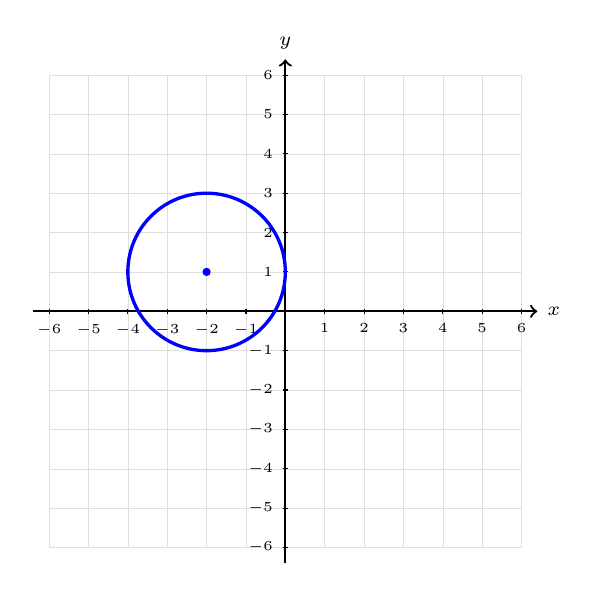
\begin{tikzpicture}[scale=0.5]
  \gridaxes{6}
  \draw[very thick,blue] (-2,1) circle (2);
  \fill[blue] (-2,1) circle (3pt);
\end{tikzpicture}
\par\vspace{9mm}\raggedright Equation: \underline{\hspace{4.5cm}}
\end{minipage}\hfill
\begin{minipage}[t]{0.48\linewidth}
\textbf{4.}\\[2pt]
\centering
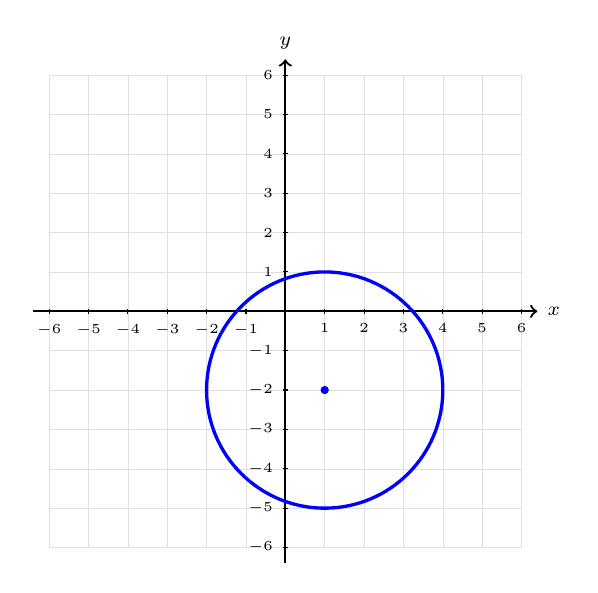
\begin{tikzpicture}[scale=0.5]
  \gridaxes{6}
  \draw[very thick,blue] (1,-2) circle (3);
  \fill[blue] (1,-2) circle (3pt);
\end{tikzpicture}
\par\vspace{9mm}\raggedright Equation: \underline{\hspace{4.5cm}}
\end{minipage}

% ===========================================================================
\newpage
\section*{Section 2 --- Circles in the Real World}

\textbf{5.}\quad \textbf{Beacon range.} A rescue beacon sits at the point $(3,4)$ on a map (units in km) and its signal reaches every point within $5$ km.

\medskip
\textbf{(a)}\quad Write an equation for the boundary of the signal's reach.

\vspace{2.5cm}
\textbf{(b)}\quad What single inequality describes all points $(x,y)$ the signal reaches?

\vspace{5.5cm}
\textbf{(c)}\quad For each camp, decide whether it is inside the signal's reach, outside it, or exactly on the boundary. Justify with a computation, not a sketch: camps at $(5,2)$, at $(9,-1)$, and at $(7,7)$. \textit{Hint: use an inequality.}

\vspace{2cm}

\newpage
\textbf{6.}\quad \textbf{Ferris wheel.} A Ferris wheel is a circle of radius $6$ m whose center is $8$ m above the ground. Put the origin on the ground directly below the center, with $y$ measuring height.

\medskip
\textbf{(a)}\quad Write the equation of the wheel.

\vspace{3cm}
\textbf{(b)}\quad What are the heights of the lowest and highest points of the wheel?

\vspace{3cm}
\textbf{(c)}\quad Cars are placed on the edge of the Ferris wheel. A car is horizontally $3$ m to the right of the center ($x = 3$), but of unknown height. Find the two possible heights of the car (exact values).

\vspace{4cm}

% ===========================================================================
\newpage
\section*{Section 3 --- Quadratic Inequality Applications}
Recap. To solve a quadratic inequality: move everything to one side, factor, and do a sign analysis of the factors. Give answers in interval notation where it fits.

\medskip
\textbf{7.}\quad \textbf{The throw.} A ball is thrown so that its height in feet after $t$ seconds is
\[
  h(t) = -16t^2 + 48t + 64 .
\]
During what time interval is the ball at height $96$ feet or above?

\vspace{7cm}
\textbf{8.}\quad \textbf{The lemonade stand, scaled up.} A stand's weekly profit from selling $x$ pitchers is
\[
  P(x) = -2x^2 + 120x - 1000 \text{ dollars.}
\]
For which values of $x$ is the profit \emph{more than} $600$ dollars?

\vspace{7cm}

% ===========================================================================
\newpage
\section*{Section 4 --- Beyond Quadratics: Applications}
Recap. With three or more factors, or factors in a denominator, track the sign of each factor on a number line. Remember: never multiply both sides by an expression whose sign you do not know, and exclude any value that makes a denominator zero.

\medskip
\textbf{9.}\quad \textbf{Average cost.} Producing $x$ gadgets costs $2x + 50$ dollars in total.

\textbf{(a)}\quad What is the average cost per gadget?
\vspace{5cm}

\textbf{(b)}\quad How many gadgets must be produced for the average cost to be at most $4$ dollars per gadget? (Remember what values of $x$ even make sense here.)

\vspace{7cm}

\newpage
\textbf{10.}\quad \textbf{The box.} A box has width $x$, length $6-x$, and height $8-x$ (all in inches), so its volume is
\[
  V(x) = x(6-x)(8-x) .
\]
\textbf{(a)}\quad Solve the inequality $V(x) > 0$ completely, using a sign chart with all three factors.

\vspace{5cm}
\textbf{(b)}\quad Your sign chart should produce \emph{two} intervals. Only one of them describes a real box. Which one, and why is the other one physically impossible even though the algebra allows it?

\vspace{3cm}

% ===========================================================================
\newpage
\section*{Section 5 --- Extra Practice}

\textbf{11.}\quad \textbf{Where a line meets a circle.} Find all points where the line $y = x + 1$ intersects the circle $x^2 + y^2 = 25$. 

\vspace{7.5cm}
\newpage
\textbf{12.}\quad \textbf{Spot the error.} A student solves $\dfrac{x+3}{x-2} \ge 1$ like this:

\begin{quote}
``Multiply both sides by $x-2$ to get $x + 3 \ge x - 2$, which simplifies to $3 \ge -2$. That is always true, so the answer is all real numbers.''
\end{quote}

\textbf{(a)}\quad Find a specific value of $x$ that shows this answer is wrong.

\vspace{4cm}
\textbf{(b)}\quad Name the exact step where the argument breaks, and explain why it is not allowed.

\vspace{4cm}
\textbf{(c)}\quad Solve the inequality correctly.

\vspace{4.5cm}

% ===========================================================================
\newpage
\section*{$\bigstar$ Challenge Problem}

\textbf{13.}\quad$\bigstar$\quad Suppose we have the equation
\[
  Ax^2 + Bx + Ay^2 + Cy = D
\]
for some constants $A, B, C, D$, where $A \neq 0$.

\medskip
\textbf{(a)}\quad Is the graph of this equation guaranteed to be a circle? If it is a circle, find its center and radius in terms of $A, B, C, D$. If it is not always a circle, determine exactly when it is one --- and describe what the graph looks like in the other cases.

\vspace{9cm}
\textbf{(b)}\quad Why was it necessary to require $A \neq 0$? What kind of graph does the equation have if $A = 0$ (and $B$, $C$ are not both zero)?

\vspace{4cm}

% ===========================================================================
\newpage
\section*{Instructor Answer Key}

\textbf{Section 1:}
\begin{itemize}\itemsep2pt
  \item 1. Center $(2,-1)$, radius $3$.
  \item 2. Complete the square: $(x-3)^2 + (y+2)^2 = 9$; center $(3,-2)$, radius $3$.
  \item 3. $(x+2)^2 + (y-1)^2 = 4$.
  \item 4. $(x-1)^2 + (y+2)^2 = 9$.
\end{itemize}

\textbf{Section 2:}
\begin{itemize}\itemsep2pt
  \item 5. (a) $(x-3)^2+(y-4)^2=25$. (b) $(x-3)^2+(y-4)^2 \le 25$. (c) $(5,2)$: $4+4=8<25$ inside; $(9,-1)$: $36+25=61>25$ outside; $(7,7)$: $16+9=25$ exactly on the boundary.
  \item 6. (a) $x^2+(y-8)^2=36$. (b) Lowest $2$ m, highest $14$ m. (c) $9+(y-8)^2=36 \Rightarrow y = 8 \pm \sqrt{27} = 8 \pm 3\sqrt3$ (about $2.8$ m and $13.2$ m).
\end{itemize}

\textbf{Section 3:}
\begin{itemize}\itemsep2pt
  \item 7. $-16t^2+48t+64 \ge 96 \Rightarrow t^2-3t+2 \le 0 \Rightarrow (t-1)(t-2)\le 0 \Rightarrow 1 \le t \le 2$; interval $[1,2]$.
  \item 8. $-2x^2+120x-1000 > 600 \Rightarrow x^2-60x+800<0 \Rightarrow (x-20)(x-40)<0 \Rightarrow 20 < x < 40$.
\end{itemize}

\textbf{Section 4:}
\begin{itemize}\itemsep2pt
  \item 9. (a) $\frac{2x+50}{x}$ dollars per gadget. (b) $\frac{2x+50}{x}\le 4 \Rightarrow \frac{50-2x}{x}\le 0$; since $x>0$, need $x \ge 25$ gadgets.
  \item 10. (a) Roots $0, 6, 8$; sign chart gives $V>0$ on $(0,6)\cup(8,\infty)$. (b) Only $(0,6)$: for $x>8$ the algebra makes $V>0$ because \emph{two} factors are negative --- but a box cannot have negative length and height. Context beats algebra.
\end{itemize}

\textbf{Section 5:}
\begin{itemize}\itemsep2pt
  \item 11. $x^2+(x+1)^2=25 \Rightarrow x^2+x-12=0 \Rightarrow (x+4)(x-3)=0$; points $(-4,-3)$ and $(3,4)$.
  \item 12. (a) E.g.\ $x=0$: $\frac{3}{-2} = -1.5 \not\ge 1$. (b) Multiplying both sides by $x-2$, whose sign is unknown --- when $x<2$ it is negative and the inequality must flip, so one multiplication cannot cover both cases. (c) $\frac{x+3}{x-2}-1 \ge 0 \Rightarrow \frac{5}{x-2} \ge 0 \Rightarrow x-2>0 \Rightarrow x>2$.
\end{itemize}

\textbf{Challenge:}
\begin{itemize}\itemsep2pt
  \item 13. (a) Divide by $A$: $x^2+\tfrac{B}{A}x+y^2+\tfrac{C}{A}y=\tfrac{D}{A}$. Complete both squares:
  \[
    \left(x+\tfrac{B}{2A}\right)^2+\left(y+\tfrac{C}{2A}\right)^2 = \tfrac{D}{A}+\tfrac{B^2+C^2}{4A^2} = \tfrac{B^2+C^2+4AD}{4A^2}.
  \]
  Not guaranteed. Let $R = \tfrac{B^2+C^2+4AD}{4A^2}$. If $R>0$: a circle with center $\left(-\tfrac{B}{2A},\,-\tfrac{C}{2A}\right)$ and radius $\sqrt{R}$. If $R=0$: a single point (the center). If $R<0$: no graph at all --- a sum of squares cannot be negative.
  \item (b) With $A=0$ there are no squared terms to complete (and the division by $A$ is illegal): the equation becomes $Bx+Cy=D$, a \emph{line}. The $A\neq 0$ condition is what guarantees the equation is genuinely quadratic in both variables with \emph{equal} coefficients --- the fingerprint of a circle.
\end{itemize}

\end{document}